%------------------------------------------------------------------------------
% Exemplo de documento para auxiliar a padronização das monografias da 
% Faculdade de Economia - UFF
%------------------------------------------------------------------------------


\documentclass[12pt, openright, chapter=TITLE]{economia} %---------------------
% Estão disponíveis opções de impressão como frente e verso, papel A4, outras
% linguagens e ets...
%------------------------------------------------------------------------------ 

\usepackage{amsmath}
\usepackage{tikz}
\usepackage{mathdots}
\usepackage{yhmath}
\usepackage{cancel}
\usepackage{color}
\usepackage{siunitx}
\usepackage{array}
\usepackage{multirow}
\usepackage{amssymb}
\usepackage{gensymb}
\usepackage{tabularx}
\usepackage{booktabs}
\usetikzlibrary{fadings}



\newtheorem{defi}{Definição}
\newtheorem{teo}{Teorema}
\newtheorem{prop}{Proposição}
\newtheorem{prova}{Demonstração}
\newcommand{\R}{\mathbb{R}}
\newcommand{\C}{\mathcal{C}}
\newcommand{\I}{\mathcal{I}}
\newcommand{\A}{\mathcal{A}}
\newcommand{\F}{\mathcal{F}}
\newcommand{\X}{\mathbf{X}}
\newcommand{\Prob}{\mathbb{P}}
\newcommand{\1}{\mathds{1}}
%------------------------------------------------------------------------------
% INFORMAÇÕES E DADOS PARA A CAPA
%------------------------------------------------------------------------------

\titulo{Efeitos Marginais em Florestas Aleatórias: Teoria, Estimação e uma Aplicação nos Acidentes em Rodovias Federais}
\autor{Pedro Cavalcante Oliveira}
\data{2019} 
\orientador{Prof. Dr. Jesus Alexei Luizar Obregon}
\coorientador{Prof. Dr. Bruno Santiago}


%------------------------------------------------------------------------------
%	FOLHA DE ROSTO E PREAMBULO
%------------------------------------------------------------------------------

\preambulo{Monografia apresentada ao curso de Bacharelado em Ciências Econômicas da Universidade Federal Fluminense como requisito parcial para conclusão do curso.}

%------------------------------------------------------------------------------
% INÍCIO DO DOCUMENTO
%------------------------------------------------------------------------------

\makeindex

\begin{document}

%------------------------------------------------------------------------------
% ELEMENTOS PRÉ-TEXTUAIS E CAPA
%------------------------------------------------------------------------------

%------------------------------------------------------------------------------
% Aqui iremos inserir, em ordem, a capa '\imprimircapa', a folha de rosto
% '\imprimirfolhaderosto*', as figuras da monografia '\figuras' e as tabelas
% 'tabelas'. É possível também a inserção de quadros, por exemplo, com o 
% comando 'quadros'. Sempre pulando uma linha entre as opções de ''listas''
%------------------------------------------------------------------------------

\imprimircapa 						
\imprimirfolhaderosto*	  					

\begin{folhadeaprovacao}

   	\pre
   
   	\vfill
   	Trabalho aprovado em 26 de Março de 2021\\
   	\banca
   	\assinatura{\textbf{\imprimirorientador}\space Orientador \\ \uff} 
   	\assinatura{\textbf{Prof. Dr. Bruno Santiago} \\ \uff} % Escrever o nome do professor
   	\assinatura{\textbf{Prof. Dr. Luciano Vereda} \\ \uff} % Se for outra instituição, escrever o nome
   	%\assinatura{\textbf{Professor} \\ Convidado 3}
   	%\assinatura{\textbf{Professor} \\ Convidado 4}
   	\vfill
	  
\end{folhadeaprovacao}	
\clearpage

% ------------------------------------------------------------------
% RESUMO E ABSTRACT
%
% Para iniciarmos um ambiente, seja de resumo, abstract ou outro 
% qualquer, devemos começar pelo \begin. Onde eu escrevo nesse 
% arquivo, já me encontro dentro de um ``ambiente de resumo''.
%
% Aqui, apresentarei o resumo e mais um outro comando de exemplo: o 
% \lipsum. A principal função do \lipsum é gerar textos aleatórios -
% textos dummys. Assim, por mais que no presente documento - 
% no arquivo .TeX - os \lipsum[3-5] ou \lipsum[2-4] apareçam, no 
% .pdf esses só aparecerão como textos aleatórios.
% ------------------------------------------------------------------

%\setlength{\absparsep}{18pt} % ajusta o espaçamento dos parágrafos do resumo
\begin{resumo}

Floresta Aleatória é um modelo de classificação estatística construído agregando de árvores de decisão, cujas aplicações práticas vão de previsão de risco de crédito e preços de ativos, à avaliação de políticas públicas, reconhecimento de padrões visuais, prevenção contra fraudes e detecção de doenças em exames médicos. Embora de uso amplo e disseminado, há pouca literatura documentando as relações sistemáticas entre variações nas variáveis explicativas e a correspondente na variável de resposta. Primeiro a teoria principal por trás da técnica é exposta, então a problemática da estimação de efeitos marginais é apresentada, uma formulação matemática e analítica do problema é encontrada e um procedimento prático de estimação e cálculo dos efeitos marginais baseado em simulações de Monte Carlo é apresentado. Por fim, um estudo de caso com dados de acidentes em rodovias federais da Polícia Rodoviária Federal estima o "Efeito Bolsonaro". 


\textbf{Palavras-chave}: Florestas Aleatórias; Classificação Estatística; Aprendizado de Máquina; Econometria Aplicada. % Palavra-chave inicia-se com maiúscula
\end{resumo}

% ------------------------------------------------------------------
% No caso do abstract, faremos a mesma coisa. Só adicionaremos a 
% opção abstract como o argumento do comando.
%-------------------------------------------------------------------

\begin{resumo}[ABSTRACT] % ESCREVER EM LETRAS MAIÚSCULAS
	


\textbf{Keywords}: Latex; Abntex; Lipsum; Economics. 	
\end{resumo}



	


\begin{dedicatoria}
	\vspace*{\fill}
	\centering
	\noindent
	\textit{Para a gata Eleonora} \vspace*{\fill}
\end{dedicatoria}
% ---

% ---
% Agradecimentos
% ---
\begin{agradecimentos}

Felizmente não falta gente a ser agradecida aqui. Da família, devo enormemente à Joana, José Carlos, Nordeval, Carmosa, Maria Helena e Luiza - sem os quais não estaria aqui, escrevendo esta monografia. Todos vocês me deram muito, muito amor.

Dos amigos que fizeram a sábia escolha de não partilhar uma graduação comigo agradeço enormemente Rômulo, Lucas, Leonardo(s), Maurício, Carolina, Marcelo, João Victor e Mauro. Obrigado pelo apoio, pelas noites e pelo carinho, tenho cada um de vocês em um lugar especial. Dos que trilharam e trilham este caminho profissional comigo, devo muito a Jamil Civitarese, que me ensinou muito mais do que econometria, Daniel Duque, que entre o início e o fim desta graduação me deu votos de confiança fundamentais nesta jornada e se tornou uma sã e necessária figura pública. Flavio Abdenur e Diego Cardoso são pessoas incríveis e para mim foram como amigáveis faróis, sempre animados em compartilhar dois centavos de experiência. Não sei dizer o que seria de mim sem Daniel Coutinho e seus aparentemente infinitos saberes. Alexandre Portugal, Leonardo Grandelle e Bruno Lopes foram presentes da UFF e a eles devo alguns dos momentos mais felizes destes últimos quatro anos.

Não foram poucos mestres nestes 22 anos de vida. José Nazareno, Diomário Silva, Ludmilla [lembrar sobrenome] e João Aprígio foram professores de escola que guardo no coração. Bruno Santiago me ajudou a trilhar o sinuoso e surpreendentemente prazeroso caminho da Matemática, sempre com um sorriso no rosto e uma paciência invejável. Jesus Obregon é talvez o maior responsável pela conclusão de graduação que se aproxima e a ele agradeço cada um dos seguidos e significantes votos de confiança. Luciano Vereda foi um excelente professor, quase me convenceu que Macroeconomia é interessante. Também cito Paulo Gusmão, Juliana Coelho, Jony Arrais e Wilson Calmon.

Tive o prazer e a sorte de ter muitas experiências práticas nestes últimos anos. Agradeço muito à equipe do Instituto Mercado Popular, onde dei os primeiros passos no mundo da análise e apresentação de dados - especialmente a Carlos Góes, André Spigariol, Pedro Menezes, Diego Cardoso e Flavio Abdenur. No Instituto de Pesquisa Econômica Aplicada do Rio de Janeiro, Felipe Russo, Maíra Franca e Carlos Henrique Corseiul. Na Fundação Getúlio Vargas, Jamil Civitarese e Amanda Medeiros. Na Análise Macro, Vitor Wilher. Na Mutual, Patrick Maia e Matheus Castro, ambos me deram um norte. 

Agradeço, por fim, a todos e todas cujos nomes não foram citados aqui, mas que participaram desta jornada, em construção até acabar. Obrigado por tudo. 


\end{agradecimentos}		
					
\figuras

\tabelas

\sumario


% -----------------------------------------------------------------------------
% ELEMENTOS TEXTUAIS
% -----------------------------------------------------------------------------

\textual



% ------------------------------------------------------------------
% Exemplo de introdução gerada por textos dummys a partir do
% lipsum
%-------------------------------------------------------------------


\chapter{Introdução}
\label{cap:intro} % faço a referência na bibliografia
\section{Motivação e Estado da Literatura}

O modelo descrito em \cite{breiman2001random} apresenta um procedimento de estimação de uma sequência de Árvores de Decisão a partir de subamostras independentes e identicamente distribuídas de um conjunto de dados. O nome da técnica vem do algorítimo consistir em montar uma coleção de Árvores de Decisão e empregar procedimentos de amostragem para que cada árvore individual seja exposta a uma subamostra aleatoriamente encontrada dos dados.

Modelos de Floresta Aleatória (no original, \texit{Random Forest}) têm aplicações em áreas variadas. Pesquisa biomédica, identificação de padrões em visão computacional, finanças e microeconomia aplicada são áreas que já difundiram seu uso. Um entendimento próprio de efeitos marginais não é importante somente para aplicações econométricas, mas também para trabalho aplicado no geral. 

Em revisões de literatura (\cite{siroky2009navigating}; \cite{biau2016random}) costuma-se enfatizar alguns resultados sobre a performance da técnica - que geralmente entrega performance preditiva elevada \citep{gu2018empirical}. Geralmente falando, com o crescimento do número de árvores o erro de previsão fora da amostra converge a zero, sua variância diminui e o custo computacional cresce com derivada decrescente. O procedimento de estimação original de Breiman fornece um estimador (i) não-viesado, (ii) consistente e (iii) factível, todas propriedades centrais na aplicabilidade dessa técnica. 

Assim como em modelos lineares, também é possível decompor variância explicada do modelo. \cite{stijven2011separating} introduziram algumas ferramentas de regressão simbólica no modelo original de Breiman para explicar importância relativa de regressores e há maneiras de abordar o mesmo problema usando Valores de Shapley, vindos da Teoria dos Jogos Cooperativos \citep{cohen2007feature}.

Avanços recentes na literatura focam em frentes diversas. Uma que dialoga com o problema a ser estudado nesta monografia é como conciliar os modelos com bancos de dados com uma quantidade crescente de variáveis e, portanto, alta dimensionalidade. Uma direção de pesquisa foca em adequar a teoria que fundamenta a técnica ao contexto em alta dimensão \citep{athey2019generalized}, outra em seleção de variáveis e redução de dimensionalidade \citep{hastie2015statistical}. 

Esse esforço de pesquisa gerou um princípio de entendimento melhor de efeitos de tratamento. \cite{ikonen2016machine} desenvolveu uma tećnica (rudimentar) de estimação de efeitos de tratamento sintéticos - uma extensão da técnica de Controles Sintéticos \citep{abadie2010synthetic}. A dupla Athey e Wager, particularmente ativa neste debate, deixou algumas contribuições importantes. Primeiro em contexto de alta dimensão \citep{athey2018approximate}. e depois em contexto de tratamentos heterogêneos \citep{wager2018estimation}. 

Em modelos lineares sabemos ser possível acomodar não-linearidades arbitrárias imputando no modelo funções não-lineares dos regressores originais. O que se mantém inalterado é a linearidade dos efeitos marginais. Em Florestas Aleatórias sabemos que por desenho não é necessário inserir funções não-lineares dos regressores para acomodar não-linearidades, então essa ponte já está estabelecida, no entanto pouco é sabido sobre o comportamento dos efeitos marginais - apesar da prolífica pesquisa no campo.

O objetivo desta monografia é propor um procedimento sistemático de estimação de efeitos marginais de tratamento, avaliar o quão (in)constantes são os efeitos marginais e o quão sensíveis aos outros regressores eles são. A metodologia empregada será estimar um modelo de Floresta Aleatória, computar suas previsões na observação mediana dos dados e em observações medianas com perturbações controladas em cada regressor. O resultado é uma curva relacionando valor predito com valores dos regressores, cuja derivada - se computável - entrega os efeitos marginais.

O cronograma esperado do trabalho segue:

\begin{table}[h]
\begin{tabular}{|l|l|l|l|l|l|l|}
\hline
Atividade / Mês                                         & 1 & 2 & 3 & 4 & 5 & 6 \\ \hline
Revisão Bibliográfica                                   & x & x & x & x &   &   \\ \hline
Desenvolvimento Teórico do Modelo e Abordagem           & x & x &   &   &   &   \\ \hline
Preparação das rotinas e programas                      &   & x & x &   &   &   \\ \hline
Análise, Interpretação e Visualização dos Resultados    &   &   & x & x &   &   \\ \hline
Redação da Monografia                                   &   &   &   &   & x & x \\ \hline
Revisão do Projeto, Reprodução e Entrega &   &   &   &   &   & x \\ \hline
\end{tabular}
\end{table}

\section{Teoria Preeliminar}

A unidade mais simples de uma Floresta Aleatória é uma Árvore de Decisão \cite{breiman2017classification} então a exposição precisa partir dessa unidade mais básica. Vamos construir uma árvore de decisão.

Uma \textbf{observação} de $k$ variáveis é um vetor $x \in \R^k$ onde cada dimensão representa uma variável diferente. Variáveis binárias podem ser representadas por pares $0$ e $1$. Definimos o \textbf{Espaço de Mensuração} $\mathbf{X}$ como sendo o conjunto de todos os vetores $x$ possíveis para os suportes definidos. Por exemplo: se um vetor representa idade, entendemos que seu suporte está nos inteiros positivos entre $0$ e, digamos, $120$. Se uma variável é uma categoria binária como sim e não, então seu suporte está em $0$ e $1$. 

As observações podem ser entendidas como pertencendo a \textbf{classes}, estando a cargo do modelador definir exatamente quais classes são essas. Dizemos que o problema é de \textbf{Classificação} quando nossas observações tem suas classes em um conjunto discreto e que o problema é de \textbf{Regressão} quando há um conjunto infinito e não-enumerável - isto é, não há um isomorfismo entre o conjunto de classes e os naturais - de classes disponíveis. Classificar um paciente como sendo portador de uma doença ou não é claramente um problema de classificação. Estimar o preço de um imóvel com base em suas características é um problema de regressão. Suponha que temos um conjunto de classes $\C = \{1,2,...,J\}$ com $J$ classes. Usaremos $\C(x)$ como a classe da observação $x$. 

\begin{defi}
Um \textbf{Classificador} é uma função $\math{C} : \mathbf{X} \to \C$.
\end{defi}

Podemos entender um Classificador de outra maneira. Defina o conjunto $A_i = \{ x \in \mathbf{X} \,\, ; \,\, \C(x) = i\}$. Então a união $\bigcup_{i = 1}^J A_i$ é o próprio conjunto $\mathbf{X}$ e cada $A_i$ é disjunto de todos os outros $A_{j \neq i}$.

\begin{defi}
Um \textbf{Classificador} é uma partição disjunta de $\mathbf{X}$.
\end{defi}

Estimar uma Floresta Aleatória (ou Árvore de Decisão, modelo de regressão linear, o que quer que seja) é fundamentalmente escolher entre as inúmeras possibilidades de Classificadores o mais apropriado para os \textbf{dados}. Os procedimentos estatísticos que empregamos para encontrar alguma aproximação desde "classificador ideal" são aplicados em algum tipo de amostra.

\begin{defi}
Uma \textbf{Amostra} de tamanho $N$ consiste de um conjunto $ A = \bigcup_{i=1}^N (x_i, \C(x_i))$ de observações empíricas.
\end{defi}

Por fim, precisamos entender a estrutura dos dados. Dizemos que se toda observação assume um vetor no $\R^k$ então dizemos que os dados têm estrutura \textbf{padrão} ou \textbf{\textit{tidy}} \cite{tidyr}. Dados não-padrão são aqueles em que há um número variável de dimensões nas observações.

\section{Construindo uma Árvore de Decisão}

Um classificador Árvore de Decisão é qualquer classificador que admita uma representação como um Grafo que é uma Árvore. Um Grafo qualquer é dito árvore se todos os seus vértices têm a propriedade de que sua remoção do grafo gera dois componentes disjuntos.

Cada divisão $D_i$ carrega duas informações: (i) um teste lógico factível para todas as observações passarem ou não (e.g. ao classificar a classe de um navio militar, nenhum com mais de $100m$ de comprimento pode ser um destróier) e (ii) uma posição na árvore.

\includegraphics[scale = .45] {avore.png}

Cada divisão quebra todas as observações que chegaram nela em exatamente dois grupos. Então toda divisão posterior gera apenas subconjuntos. Uma divisão pode ser de dois tipos: terminal e não-terminal. Se uma divisão implica classificação perfeita (todas as observações que atendem ao critério são da mesma classe), então não há por que continuar a dividir os dados e esta divisão termina seu "galho" da árvore. 

\section{Noções de Estimação de uma Árvore de Decisão}

Como podemos traduzir uma amostra $A$ em uma árvore de decisão $\A$? Um dos procedimentos mais consagrados, apresentado na primeira edição de \cite{breiman2017classification} será apresentado.

Primeiro definimos a \textbf{Proporção} de um vértice como um vetor contendo a proporção de cada classe observada nos dados que chegaram ao vértice. Depois, a \textbf{Impureza} do nodo. A função $\I(\cdot)$ mapeia um nodo em um número positivo limitado superiormente por um real $I$ de forma que a impureza de um nodo cuja proporção seja igual para todas as classes seja $0$ e a impureza de um nodo cuja proporção seja unitária para alguma classe seja $I$. Precisamos impor apenas que $\I(\cdot)$ seja monotonamente crescente em relação à probabilidade de cada classe. O valor específico da impureza não é relevante, desde que aumente monotonamente em relação à heterogeneidade de proporções observadas.

Tome uma divisão $D_i$ qualquer. Ela rende duas subamostras/divisões que podem ou não serem terminais, $D_{iA}$ e $D_{iB}$. Defina $P_A (D_i)$ como a proporção de casos que chegam em $D_i$ e vão para $D_{iA}$ e o mesmo para $P_B (D_i)$.

\begin{defi}
A \textbf{Qualidade} da divisão é dada pela variação na impureza: $\mathcal{Q} (D_i) := \I(D_i) - P_A(D_i) \I (D_{iA}) - P_B(D_i) \I (D_{iB})$.
\end{defi}

 Escolher a divisão adequada envolve muitos recursos computacionais e selecionar a divisão que maximize a qualidade dentre as potenciais. Qualquer regra computável pode ser usada: um valor ser maior ou menor que um certo patamar, estar em uma certa faixa, etc. Os aspectos algorítmicos deste problema são interessantes porém fogem ao escopo desta monografia, discussões podem ser encontradas em \cite{de1991distance}.
 
 \section{Construindo uma Floresta Aleatória}
 
 A agregação das predições de árvores construídas a partir de pedaços diferentes da amostra é um passo seguinte e natural à modelagem anteriormente apresentada. Como os procedimentos de escolha de nodos/divisões são largamente estocásticos, árvores individuais de decisão podem apresentar vieses ou baixa performance ao acaso. Se um número grande de árvores é agregado e não há relação sistemática do erro de predição com alguma variável preditiva, então os erros devem se anular com o aumento do número de árvores.
 
 \begin{defi}
 Uma \textbf{Floresta Aleatória} é um conjunto $\F = \{\A_1, \A_2,...,\A_k\}$ de árvores de decisão de forma que dada uma amostra $A$ existe um conjunto de subamostras únicas $B = \{ B_1, B_2, ..., B_k\}$ independentes e $\A_i$ foi treinada na amostra $B_i$.
  \end{defi}
  
  \begin{defi}
  A \textbf{Margem} de uma floresta, dada uma observação $\X$ e um vetor aleatório de amostragem $Y$ é a função $M(\F, \X, Y)= \sum_{i=1}^k \1 ( \A_i (\X) = \C(\X) ) - \sum_{i=1}^k \1  ( \A_i (\X) \neq \C(\X) )  $ onde $\1(\cdot)$ é a função indicadora.
  \end{defi}
  
  A margem provê uma medida do quão precisa é a floresta em votar corretamente na classe verdadeira da observação. Uma margem maior sinaliza uma maior capacidade da floresta de discriminar observações. Note que a Margem de uma floresta é uma variável aleatória hierárquica. Idealmente a variância condicional ao vetor de amostragem é aproximadamente constante e averiguar se não há mudanças sistemáticas nos resultados para vetores de amostragem diferentes é parte do trabalho de avaliação de qualquer floresta estimada. Definimos o \textbf{Erro de Generalização} como $G(\F, \X, Y) := \Prob (M(\F, \X, Y)) < 0)$, a probabilidade de que a margem seja negativa, a previsão da floresta esteja errada. 
 
 Um resultado fundamental sobre Florestas Aleatórias é de que não há aumento do erro de generalização com a adição de árvores. O comportamento é de limitação do erro de generalização.
 
 \begin{teo}[Convergência do Erro de Generalização]
 Defina a sequência $E_k = \{ G(\F_k, \X, Y) \}$ de forma que $\F_k$ seja apenas $\F_{k-1}$ com a $k$-ésima árvore adicionada. Tome as classes possíveis $\C = \{1,2,3,..,i,j,...,J \}$. Suponha que $\C(\X) = i$. Então $E_k \to \sum_{i=1}^k \1 ( \A_i (\X) = i ) - \underset{i \neq j}{\text{Max}} \sum_{i=1}^k \1  ( \A_i (\X) = j ) $
 
 \end{teo}
 
 \begin{prova}
 Ver o Apêndice 1 de \cite{breiman2001random}. \blacksquare
 \end{prova}
 
 \section{Organização da Monografia}
 
 Vimos como uma árvore de decisão pode distinguir observações e captar não-linearidades no processo gerador. Depois, que agregar árvores pode produzir uma espécie de mitigação de viés que uma árvore individual possa ter, construímos uma maneira de medir o quão bem o processo de voto democrático de cada árvore da floresta discrimina observações com sua Margem e que a partir dela podemos computar uma medida da performance preditiva em dados que não foram apresentados ao modelo em sua fase de treinamento. Por fim, vimos que o erro de generalização com dados desconhecidos tem um limite superior dado um aumento do tamanho da floresta. Estes são os fatos básicos do funcionamento do modelo.
 
 O capítulo 2 desenvolve mais a teoria por trás das principais propriedades de Florestas Aleatórias, o capítulo 3 apresenta o algorítimo de computação dos efeitos marginais e o desenho da simulação. O capítulo 4 apresenta algumas estatísticas descritivas dos dados e as estimativas da Floresta. O capítulo 5 mostra as simulações e a computação dos efeitos marginais em si. O capítulo 6 conclui com alguns fatos estilizados.



\chapter{Florestas Aleatórias}

\section{Propriedades}

\section{(Quase-)Inferência}

\section{Estimação}


\section{Validação}
\subsection{Validação Dentro-Fora da Amostra}
\subsection{Validação Cruzada}

\chapter{Computação de Efeitos Marginais}
\section{Modelos Lineares}
\subsection{Modelando Não-Linearidades com Modelos Lineares}
\subsection{Efeitos Marginais em Modelos Lineares}
\section{Dependência Parcial para Florestas Aleatórias}
\section{Preenchimento de Suporte}

\chapter{Dados, Estimação e Validação}s


%% ------------------------------------------------------------------
% Aqui, o objetivo é mostrar como colocar uma imagem ou um gráfico 
% na presente monografia. tudo que faremos é usar um ambiente 
% gráfico e assim, iremos o gerar. 
%-------------------------------------------------------------------

%-------------------------------------------------------------------
% Novamente, para preenchermos o documento, usaremos o lipsum
%-------------------------------------------------------------------

\chapter{Conceitos Matemáticos}
Esta monografia está permeada de argumentos matemáticos formais, de fato é a sua contribuição central. Como os requisitos matemáticos ao seu entendimento são um tanto quanto específicos, aqui faço uma breve exposição da teoria necessária ao entendimento com um grau adequado de rigor. Tratamentos mais ou menos rigorosos existem em abundância e as duas principais referências são \cite{rudin} e \cite{pugh}.

Alguns cuidados com definir apropriadamente corpos, operações de soma e multiplicação foram omitidos. É do meu entendimento que uma concepção operacional não-rigorosa destes conceitos é suficiente para os propósitos desta monografia.

Dividi essa seção em quatro partes. Em \ref{primeira} cubro alguns aspectos básicos como métricas e sequências, culminando na demonstração de que o $(\mathbb{R}^k, d)$ é um espaço métrico completo se $d(.,.)$ for uma métrica plena. Em \ref{segunda} abordamos Topologia Ponto-a-Conjunto com um grande enfoque nos reais. O fato central que esta seção trará será o teorema de Bolzano-Weierstrass. As ferramentas descobertas nessa seção serão de enorme uso ao longo de toda esta monografia. Em \ref{terceira} abordaremos funções e alguns resultados de teoria de ponto fixo. Na \ref{quarta} concluímos este pequeno curso relâmpago ao abordar espaços de funções e equações diferenciais.


\section{Sequências, Espaços Métricos e Completude}
\label{primeira}


\subsection{Métricas}

Uma discussão interessante sobre processos estocásticos requer uma bem definida noção de distância. Afinal, o que faz dois elementos \textit{distarem} um do outro e como mediremos isso? Imagine um conjunto $X$ como quiser. Um disco, os reais, um contorno de pato no plano cartesiano... 

\begin{defi}
Uma \textbf{métrica} é uma função $d: X \times X \to \mathbb{R}$ que atende quatro propriedades:

\begin{itemize}
    \item \textbf{Simetria:} $d(x,y) = d(y,x)$. 
    \item \textbf{Unicidade:} $d(x,x) = 0$.
    \item \textbf{Positividade:} $d(x,y) \geq 0$
    \item \textbf{Desigualdade Triangular:} $d(x,y) \leq d(x,z) + d(z,y)$. 

\end{itemize}
\end{defi}

Observe que as três primeiras propriedades que estamos exigindo de uma métrica apenas formalizam nossa intuição sobre como distâncias se comportam no mundo real. Ir de um lugar ao outro deve cobrir a mesma distância que a volta se usarmos a mesma rota. A distância de um ponto até ele mesmo é nula (quanto você, leitor, precisa andar para ficar parado?) e distâncias negativas seriam coisas no mínimo curiosas.

A Desigualdade Triangular é definitivamente a propriedade mais interessante de uma métrica. Ela essencialmente diz que não existem "atalhos" em um contexto em que existem distâncias. A distância entre dois pontos quaisquer sempre é no mínimo a mesma que a soma das distâncias entre estes mesmos pontos e um terceiro. Em um contexto de plano cartesiano este fato é rapidamente visualizado com a ajuda de um triângulo. 

\begin{center}
\tikzset{every picture/.style={line width=0.75pt}} %set default line width to 0.75pt        

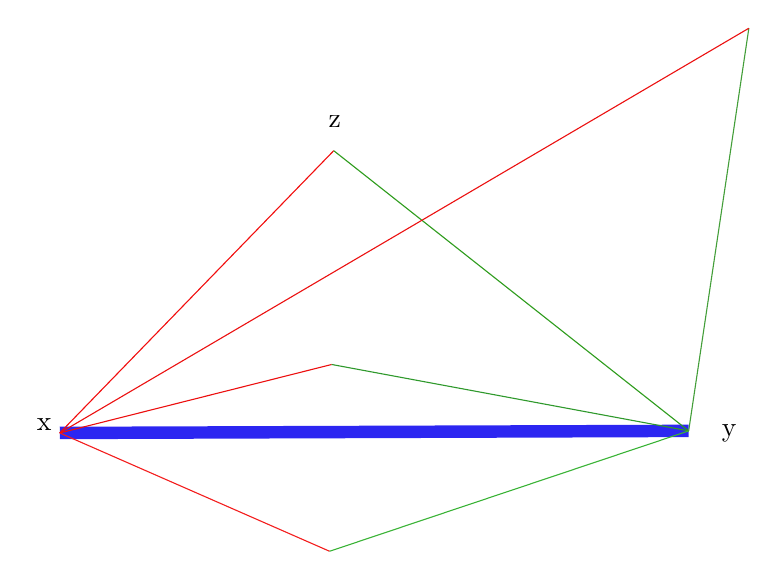
\begin{tikzpicture}[x=0.75pt,y=0.75pt,yscale=-1,xscale=1]
%uncomment if require: \path (0,300); %set diagram left start at 0, and has height of 300

%Straight Lines [id:da6847309088840179] 
\draw [color={rgb, 255:red, 44; green, 38; blue, 241 }  ,draw opacity=1 ][line width=4.5]    (69.5,214) -- (372.5,213) ;


%Straight Lines [id:da46426148005512835] 
\draw [color={rgb, 255:red, 241; green, 13; blue, 13 }  ,draw opacity=1 ]   (201.5,78) -- (69.5,214) ;


%Straight Lines [id:da2906024541588399] 
\draw [color={rgb, 255:red, 46; green, 156; blue, 29 }  ,draw opacity=1 ]   (201.5,78) -- (372.5,213) ;


%Straight Lines [id:da6028165286195768] 
\draw [color={rgb, 255:red, 236; green, 15; blue, 15 }  ,draw opacity=1 ]   (69.5,214) -- (200.5,181) ;


%Straight Lines [id:da6610711832317098] 
\draw [color={rgb, 255:red, 47; green, 153; blue, 44 }  ,draw opacity=1 ]   (200.5,181) -- (372.5,213) ;


%Straight Lines [id:da7902181564457826] 
\draw [color={rgb, 255:red, 243; green, 29; blue, 29 }  ,draw opacity=1 ]   (69.5,214) -- (199.5,271) ;


%Straight Lines [id:da8016282193076851] 
\draw [color={rgb, 255:red, 58; green, 179; blue, 54 }  ,draw opacity=1 ]   (372.5,213) -- (199.5,271) ;


%Straight Lines [id:da6023664239656019] 
\draw [color={rgb, 255:red, 67; green, 158; blue, 57 }  ,draw opacity=1 ]   (401.5,19) -- (372.5,213) ;


%Straight Lines [id:da5175708881441581] 
\draw [color={rgb, 255:red, 235; green, 17; blue, 17 }  ,draw opacity=1 ]   (401.5,19) -- (69.5,214) ;



% Text Node
\draw (62,210) node  [align=left] {x};
% Text Node
\draw (392,214) node  [align=left] {y};
% Text Node
\draw (202,64) node  [align=left] {z};


\end{tikzpicture}
\label{desitri}
\end{center}




Na figura \ref{desitri} a desigualdade triangular é clara. Em qualquer um dos triângulos, a soma do comprimento das arestas vermelha e verde é sempre menor que a azul. Existem variadas métricas, apresento aqui alguns exemplos:

\begin{itemize}
    \item \textbf{Métrica Euclidiana:} $d(x,y) = \sqrt{\sum_{i=1}^k (x_i - y_i)^2}$. Esta é a noção usual de distância que temos. Com esta métrica, o menor trajeto entre dois pontos sempre é uma reta. Observe que em uma dimensão a métrica euclidiana é simplesmente $x-y$. Em duas é o tamanho da hipotenusa do triângulo retângulo inscrito nos dois pontos. Em três é o tamanho da diagonal do cubo inscrito nos pontos e por aí vai.
    \item \textbf{Métrica Discreta:} $d(x,y) = \mathbb{1}(x \neq y)$. Uma noção um pouco curiosa de distância em que se dois elementos são diferentes dizemos que distam uma unidade. 
    \item \textbf{Métrica "Taxista":} $d(x,y) = \sqrt{\sum_{i=1}^d (x_i - y_i)}$
\end{itemize}



\subsection{Espaços Métricos}

\begin{defi}
Um \textbf{Espaço Métrico} é uma dupla de um conjunto $X$ e uma métrica $d$. Nos referimos ao espaço munido deste ambiente e dessa noção de distância como $(X,d)$.
\end{defi}

Esse conceito é mais fino e amplo do que parece à primeira vista. Estamos falando de conjuntos, então meras coleções de elementos, e de métricas, maneiras de medir distâncias. Digamos que estamos no plano cartesiano. Um conjunto qualquer prontamente se torna um espaço métrico ao munirmos ele de uma métrica - Euclidiana, discreta ou que for - e agora ganhamos espaço de manobra para garantir que certos fenômenos ocorram nele.

O poder de pensar em termos de Espaços Métricos com tanta generalidade é que conseguimos ver com mais clareza o que há de comum entre o plano cartesiano e a superfície arredondada da terra - e como espaços diferentes podem por vezes pedir métricas diferentes para responderem problemas de ordem mais prática. Conceber distância como a reta que liga dois pontos faz muito sentido no plano cartesiano ou no $\mathbb{R}^k$, mas nem tanto ao falar da superfície da terra, em que normalmente modelamos a distância entre dois pontos como o menor arco na superfície que ligue-os. 




\subsection{Sequências e Limites}


\begin{defi}
Uma \textbf{sequência} $x:\mathbb{N} \to \mathbb{R}^k$ é uma função que mapeia os naturais em elementos de algum conjunto. Podemos, alternativamente, entender uma sequência como um conjunto $\{x_n\} = \{ x_n \in \mathbb{R}^k \,\, | \,\, n \in \mathbb{N}\}$. Dizemos que uma sequência tem \textbf{limite} em $L$ - alternativamente que $L$ é limite de $x_n$ ou que $x_n$ \textbf{converge} a $L$ - se $\forall \,\, \epsilon > 0 \,\, \exists \,\, n' \in \mathbb{N} \,\, | \,\, n > n' \implies d(x_n, L) < \epsilon$. Notamos $\lim_{n \to \infty} x_n = L$
\end{defi}

Sequências são apenas conjuntos de elementos com um processo definidor. Imagine por exemplo a sequência contida na reta real $x_n = \frac{1}{n}$, ou uma prima não-muito-distante contida no $\mathbb{R}^2$, $y_n = (\frac{1}{n}, \frac{10}{n})$. Observe que $\lim x_n = 0$ e que $\lim y_n = (0,0)$. Podemos construir uma infinidade de outros exemplos, seguem alguns - todos com a métrica euclidiana em mente.

\begin{itemize}
    \item $x_n = (1 + \frac{1}{n})$ \implies 
    $\lim x_n = 1$ 
    \item $x_n = (1, 2n, \frac{79}{n})$ \implies
    $\lim x_n = (1, \infty, 0)$
    \item $x_n = \sin{n}$ \implies
    $\nexists \lim x_n$
    \item $x_n = (1+\frac{1}{n})^n$ \implies $\lim x_n = e$
    \item $x_n = (-\frac{4n^2}{3n}, n, \pi)$ \implies $\lim x_n = (-\infty, \infty, \pi)$
    \item $x_n = 2$ \implies $\lim x_n = 2$
\end{itemize}


Aos nos referir a números arbitrariamente pequenos como $\epsilon > 0$ estamos tão somente dizendo que não importa o quão arbitrariamente próximo de um ponto limite quer-se chegar, se uma sequência converge a este limite, existe algum índice natural tal que a sequência está à uma distância menor que $\epsilon$ deste limite. Observe que não importando qual natural seja escolhido, a rigor, $\frac{1}{n}$ jamais será de fato igual a zero e sim à grandezas arbitrariamente pequenas. No entanto, dada uma distância arbitrária do zero, sempre podemos atingi-la com este sequência que tenha limite em zero ao escolher um $n$ suficientemente grande. Esta é a noção de limite.

Talvez agora comece a fazer um pouco mais de sentido a escolha deliberada de falar com generalidade de distâncias. $x_n = 1/n$ por exemplo tem limite em $0$ na métrica euclidiana, mas na discreta não.

\subsection{Sequências de Cauchy}

Temos agora um pequeno problema teórico em mãos. A depender da métrica, algumas sequências cujos termos se aproximam arbitrariamente de certos pontos podem ou não ter limites. Como lidamos com isso? Abriremos mão da noção de limite e focaremos no comportamento em si: termos de uma sequência que estão cada vez menos distantes entre si.

\begin{defi}
Uma sequência é \textbf{de Cauchy} se $\forall \,\, \epsilon > 0 \,\, \exists \,\, n \in \mathbb{N} \,\, | \,\, a,b > n \implies d(x_a,x_b) < \epsilon$.
\end{defi}

Uma sequência de Cauchy apresenta essa propriedade de que para qualquer distância arbitrária de $0$ que se escolha, existe algum ponto a partir do qual todos os termos da sequência distam no máximo essa distância arbitrária, por menor que seja. Uma sequência de Cauchy é, no português mais direto, uma em que os termos subsequentes estão sempre cada vez mais próximos.

Essa noção pode ser difícil de diferenciar de uma sequência que tem limite em algum ponto então façamos um pequeno exercício mental. Imagine que estamos no espaço métrico $(\mathbb{Q}, d)$. Imagine agora a seguinte sequência:

$$a_1 = 3$$
$$a_2 = 3,1$$
$$a_3 = 3,14$$
$$a_4 = 3,141$$
$$a_5 = 3,1415$$
$$a_6 = 3,14159$$
$$...$$
$$a_{30} = 3,1415926535 8979323846 2643383279$$
$$...$$

Eu espero que seja claro ao leitor que essa sequência $a_n$ é de Cauchy. O que não pode parecer claro a princípio é que, apesar disso, não existe limite para essa sequência. Isto porque ela se aproxima arbitrariamente de $\pi$ e estamos no espaço métrico $(\mathbb{Q}, d)$. Esta sequência está indo \textbf{para fora} do espaço -  porque $\pi$ é um número irracional - ainda que seja de Cauchy e tenha termos cada vez mais próximos uns dos outros. 

\subsection{Espaços Métricos Completos}

Note que se descrevermos uma sequência de Cauchy em um espaço que esteja se aproximando de um elemento desse mesmo espaço, ela necessariamente converge, temos um limite. Será então que existem espaços em que \textbf{toda} sequência de Cauchy converge? Já sabemos que isso claramente não procede para espaços $(\mathbb{Q}, d)$, qualquer que seja a métrica.

Voltemos ao exemplo da sequência $a_n$ que se aproximava de $\pi$. Se fizermos uma operação de "colar" esse buraco faltando nos reais, a história muda. Imagine o conjunto $A = \mathbb{Q} \bigcup \{\pi\}$. Se estivermos no espaço $(A,d)$ então $\exists \lim a_n$ e mais ainda, $\lim a_n = \pi$. Isso nos deixa agora com outra infinidade de sequências que são de Cauchy e não convergem no espaço $(A,d)$ porque se aproximam arbitrariamente de números irracionais como $e$ e $\sqrt{2}$. Repetindo a operação de colar os irracionais até que tenhamos colado todos faz com que $A = \mathbb{Q} \bigcup \mathbb{I}$. 

Perceba que a união dos racionais com os irracionais dá o conjunto dos números reais e que por construção qualquer sequência de Cauchy em um espaço $(\mathbb{Q} \bigcup \mathbb{I}, d)$ converge. É impossível construir uma sequência de Cauchy de números reais que não tenha como limite outro número real. Em um espaço métrico construído com números reais, \textbf{toda} sequência de Cauchy converge. Este fato é notável e merece uma conceitualização própria.

\begin{defi}
Um espaço métrico $(X,d)$ é \textbf{completo} se nele toda sequência de Cauchy converge.
\end{defi}

Os Reais caracterizam um espaço métrico completo. Ao contrário do que ocorre nos Irracionais e nos Racionais, ambos permeados de "buracos". Completude é uma propriedade muito interessante de espaços métricos e veremos mais à frente que ela é central para a validade de alguns teoremas extremamente úteis como o do Ponto Fixo de Banach. 

Recapitulando, começamos esta seção falando de métricas. Apenas formalizamos nossa intuição sobre o que significam distâncias. A partir daí construímos um novo conceito, o de sequências e vimos que sequências são maneiras de nos aproximarmos de números de maneiras arbitrárias. Vimos depois que a depender de qual conjunto usamos para construir nossos espaços métricos, se aproximar arbitrariamente de um ponto não quer dizer convergir a ele. Por isso refinamos nosso conceito de sequência e conhecemos as sequências de Cauchy. Logo uma pergunta absolutamente natural emergiu. Queríamos saber se existem espaços em que ter um limite e ser uma sequência de Cauchy são sinônimos. Por serem "especiais" nesse sentido, demos a eles um nome específico: espaços métricos completos. E assim o são por não terem os "buracos" que racionais e irracionais têm.

Agora voltamos nossas miras para a topologia elementar ponto-a-conjunto, onde estudaremos as propriedades mais gerais de conjuntos e de espaços. 

\section{Topologia Ponto-a-Conjunto Elementar}
\label{segunda}




\subsection{Interioridade e Abertura}
\subsection{Vizinhanças e Bolas}
\subsection{Aderência e Proximidade}
\subsection{Limitação e Compacidade}
\subsection{Teorema de Bolzano-Weierstrass}


\section{Funções, Continuidade e Pontos Fixos}
\label{terceira}
\subsection{Mapa, função, transformação, campo ou correspondência?}
\subsection{Compacidade e Continuidade}
\subsection{Homeomorfismos, Retrações, Contrações e outras formas de deformar espaços}
\subsection{Um brevíssimo passeio pelos Teoremas de Ponto Fixo}
\subsubsection{Os Teoremas de Brouwer e Kakutani: Deformando Conjuntos Convexos}
\subsubsection{O Teorema do Ponto Fixo de Banach: Contraindo Espaços Completos}



\section{Mapeando Espaços de Funções}
\label{quarta}
\subsection{Espaços de Funções}
\subsection{Equações Diferenciais como Mapas do Espaço de Funções}
\subsection{Equações em Diferenças e Mapas Iterados}


\chapter{Processos Estocásticos}

Aqui faço uma exposição breve, autocontida e razoavelmente formal do objeto central deste estudo.


\begin{defi}

Um \textbf{Processo Estocástico n-dimensional} é uma sequência  $\{X_t\}_{t \in T} \subset \Omega \subseteq \mathbb{R}^n$ onde $X_t$ é uma variável aleatória e o conjunto $T = \{1,2,...,t\}$ indexa a passagem do tempo.  
\end{defi}

Confrontados com dados do mundo real, observamos apenas \textbf{uma} realização particular do processo qualquer que comande o fenômeno estudado. Logo, ao descrever a realização do processo como uma sequência, ela necessariamente caracterizará um subconjunto próprio do espaço amostral $\Omega$. 

\section{Processos Autoregressivos}

%-------------------------------------------------------------------
% O que faremos abaixo é incluir uma imagem (formato JPG, mas 
% poderia ser outro formato) no pdf. O argumento width=\textwidth 
% ajusta a largura da imagem a largura da página
%-------------------------------------------------------------------

%\begin{figure}[h]
%	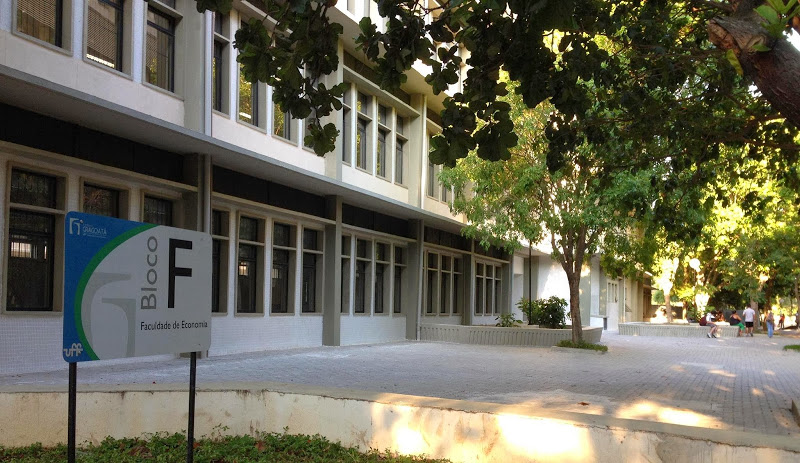
\includegraphics[width=\textwidth%]{imagens/blocof.jpg}
%	\caption{O Bloco F}
%	\label{fig:blocof} % Aqui %'nomeamos' o gráfico
%\end{figure}

%-------------------------------------------------------------------
% mais lipsum...
%-------------------------------------------------------------------


% ------------------------------------------------------------------
% Aqui, o objetivo é mostrar como colocar uma tabela. Recomenda-se,
% quando necessário, a consulta no seguinte site:
%
%                https://www.tablesgenerator.com/
%
% Em que é possível criar suas próprias tabelas na mão, ou mesmo 
% importar do excel, por exemplo..
%-------------------------------------------------------------------

\chapter{tabelas}
\label{cap:tabelas}

%-------------------------------------------------------------------
% O que faremos abaixo é incluir uma tabela num ambiente table:
%-------------------------------------------------------------------

Criaremos uma tabela simples utilizando o ambiente tabular. Com o ambiente center, iremos centralizar:



\begin{table}[h!]
	\centering
	\caption{Exemplo de Tabela}
	\begin{tabular}{l c c c} 
	    \hline
		Linha 	& Valor 1 	& Valor 2 	& Valor 3 \\ \hline 
		1 		& 6 		& 87837 	& 787 \\ 
		2		& 7			& 78 		& 5415 \\
		3 		& 545 		& 778		& 7507 \\
		4 		& 545 		& 18744 	& 7560 \\
		5 		& 88 		& 788 		& 6344 \\
		\hline
	\end{tabular}
	\label{table:1} % Aqui 'nomeamos' a tabela
\end{table}

Obviamente, podemos criar tabelas maiores e mais robustas. Nosso objetivo aqui, entretanto, não é esse. Que fique claro que outras \textit{N} possibilidades estão disponíveis. Segue um outro exemplo, feito diretamente utilizando a linguagem R:

\begin{table}[!htbp] \centering 
	\caption{Ajustes nos parâmetros} 
	\label{} 
	\begin{tabular}{@{\extracolsep{5pt}}lccc} 
		\\[-1.8ex]\hline 
		\hline \\[-1.8ex] 
								& \multicolumn{3}{c}{\textit{Dependent variable:}} \\ 
		\cline{2-4} 
		\\[-1.8ex] 				& \multicolumn{2}{c}{Overall Rating} 	& High Rating \\ 
		\\[-1.8ex] 				& \multicolumn{2}{c}{\textit{OLS}} 		& \textit{probit} \\ 
		\\[-1.8ex]				& (1) 			& (2) 					& (3)\\ 
		\hline \\[-1.8ex] 
		Handling of Complaints 	& 0.692$^{***}$ & 0.682$^{***}$ 		&  \\ 
								& (0.149) 		& (0.129) 				&  \\ 
		No Special Privileges 	& $-$0.104 		& $-$0.103 				&  \\ 
								& (0.135) 		& (0.129) 				&  \\ 
		Opportunity to Learn 	& 0.249 		& 0.238$^{*}$ 			& 0.164$^{***}$ \\ 
								& (0.160) 		& (0.139) 				& (0.053) \\ 
		Performance-Based Raises& $-$0.033 		& 						&  \\ 
								& (0.202) 		&  						&  \\ 
		Too Critical			& 0.015 		&  						& $-$0.001 \\ 
								& (0.147)		&  						& (0.044) \\ 
		Advancement 			&  				&  						& $-$0.062 \\ 
								&  				&  						& (0.042) \\ 
		Constant 				& 11.011 		& 11.258 				& $-$7.476$^{**}$ \\ 
								& (11.704) 		& (7.318) 				& (3.570) \\ 
		\hline \\[-1.8ex] 
		Observations 			& 30 			& 30 					& 30 \\ 
		R$^{2}$ 				& 0.715			& 0.715 				&  \\ 
		Adjusted R$^{2}$ 		& 0.656 		& 0.682 				&  \\ 
		Akaike Inf. Crit. 		& 				&  						& 26.175 \\ 
		\hline 
		\hline \\[-1.8ex] 
		\textit{Note:}  		& \multicolumn{3}{r}{$^{*}$p$<$0.1; $^{**}$p$<$0.05; $^{***}$p$<$0.01} \\ 
	\end{tabular} 
	\label{table:2}
\end{table} 


%-------------------------------------------------------------------
% mais lipsum...
%-------------------------------------------------------------------

\lipsum[2-4]


%-------------------------------------------------------------------
% Aqui mostraremos, por fim, como realizar uma citação
%-------------------------------------------------------------------

\chapter{Como Citar}
\label{cap:cite}

Supondo que desejássemos realizar uma citação no texto, por exemplo do pacote que usamos para fazer esse modelo de monografia. Tudo que teríamos que fazer seria utilizar o comando \texttt{citeonline\{\}} ou o \texttt{cite\{\}}. Usando o ambiente de citação, teríamos abaixo o exemplo.\cite{osbourne2009ozzy}

\begin{citacao}
	``Exemplo de um ambiente de citação. Não usamos o comando \texttt{citeonline\{\}}. Então, ao fim do ambiente iremos usar, entre parênteses para simular uma citação em ABNT.'' 
\end{citacao}


\chapter{Conclusões}
\label{cap:conclusoes}

Foi demonstrado como construir uma floresta aleatória partindo de primeiros princípios. Depois, através de notação matricial clássica no campo, como e o que são modelos lineares. A problemática de estimar efeitos marginais foi apresentada e um procedimento computacionalmente simples para isso em seguida, demonstrando como algumas nuances passavam batido por modelos lineares.

O tema é relevante em dois sentidos. Do ponto de vista do aprendizado de máquina, porque encaixa em uma agenda maior de pesquisa em \textit{interpretabilidade} de Machine Learning. O núcleo duro reduzido da disciplina abre espaço para uma série de más práticas disseminadas no uso dessas técnicas \cite{flach2019performance}. Avaliar efeitos marginais pode ser usado como uma forma de validação qualitativa também. Relações com sinais inversos ao esperado podem ser sinal de problemas.

Há também, pelo mesmo motivo, dificuldade de comunicação de resultados de modelos e até mesmo responsabilização civil-criminal quanto às consequências de seu uso em ambiente de produção, sem supervisão humana \cite{lepri2018fair}. Interpretação de modelo, em particular antes de entrega para algum ambiente de produção em que seus resultados afetarão desde experiência de uso em aplicativos de jogos à possivelmente investigação criminal, é crucial. O economista se preocupa com interpretabilidade porque é, de certa maneira, a finalidade principal do trabalho aplicado de métodos quantitativos. Estimar efeitos marginais, (semi)elasticidades e grandezas similares representa a esmagadora maioria das aplicações de econometria, salvo raros estudos como \citeonline{edison2020text} que usam técnicas não-supervisionadas vindas de Linguística Computacional.

Uma limitação não-resolvida da técnica é a inferência dos efeitos marginais computados. É possível distingui-los estatisticamente de zero com algum teste de hipótese? Isso equivale a estabelecer uma ponte entre as duas culturas de \citeonline{breiman2001statistical}. Não parece um problema intratável. Se florestas aleatórias têm distribuição normal e estimamos várias, então temos dados e podemos fazer inferência se conhecermos a variância da floresta. Não é um problema trivial, mas está ao alcance da pesquisa. Essa avenida de pesquisa é provavelmente a de maior interesse ao econometrista aplicado e parte diretamente dos princípios elaborados nesta monografia.









% ----------------------------------------------------------
% ELEMENTOS PÓS-TEXTUAIS
% ----------------------------------------------------------
\postextual

% ----------------------------------------------------------
% Referências bibliográficas
% ----------------------------------------------------------

\nocite{abntexmanual, 
		abntex2modelo} % aqui citamos os autores que não foram citados no texto.

\bibliography{referencias}


\end{document}
